\documentclass[oneside]{unilasalle}

\usepackage[T1]{fontenc}
\usepackage{float}
%\usepackage[latin1]{inputenc}
\usepackage[utf8]{inputenc}
\usepackage{latexsym}
%\usepackage[english,brazil]{babel}
\usepackage{psfrag}
\usepackage{amssymb}
\usepackage{subfig}

\title{Integração do Sistema AppMan de Gerenciamento de Aplicações para Ambiente de Grade com diferentes Sistemas de Gerenciamento de Recursos}
%\title{Integração do Sistema AppMan de Gerenciamento}

\author{Bernardo}{Tonismar Régis}

\advisor[Profa.~DSC.]{Mangan}{Patrícia Kayser Vargas}

\course{Ciência da Computação}

\keyword{computação em grade}
\keyword{gerenciamento de recurso}
\keyword{drmaa}

\begin{document}
    %------------------------------------------------------------------------------------------------
% \simb[entrada na lista de s�mbolos]{s�mbolo}:
%   Escreve o simbolo no texto e uma entrada na Lista de S�mbolos.
%   Se o par�metro opcional e omitido, usa-se o par�metro obrigat�rio.
%------------------------------------------------------------------------------------------------
\newcommand{\simb}[2][]{%
  \ifthenelse{\equal{#1}{}}
    {\addcontentsline{los}{simbolo}{\ensuremath{#2}}}
    {\addcontentsline{los}{simbolo}{#1}}
  \ensuremath{#2}
}

\makeatletter
%------------------------------------------------------------------------------------------------
% \listadesimbolos: comando que imprime a lista de simbolos
%------------------------------------------------------------------------------------------------
\newcommand{\listadesimbolos}{
  \pretextualchapter{Lista de S�mbolos}
  {\setlength{\parindent}{0cm}
   \@starttoc{los}}}

\newcommand\listabbrname{Lista de S\'imbolos e Abreviaturas}
\newcommand\listofabbreviations{%
    \chapter*{\listabbrname
      \@mkboth{\MakeUppercase\listabbrname\space\draftdate}%
              {\MakeUppercase\listabbrname\space\draftdate}}%
     % \addcontentsline{toc}{chapter}{\MakeUppercase\listabbrname}%
    \@starttoc{lob}%
    }
\newcommand\abbrev[2]{%
                                        \def\({$}%
                                        \def\){$}%
      \addcontentsline{lob}{section}{%
                                                                \rm%
                        \protect\parbox[t]{.2\textwidth}{\bf #1}%
                   \hspace{0.025\textwidth}%
                   \protect\parbox[t]{.6\textwidth}{#2}%
        \vspace{2mm}\hspace{.1\textwidth}}%
      }

%------------------------------------------------------------------------------------------------
% como a entrada ser� impressa
\newcommand\l@simbolo[2]{\par #1, p.\thinspace#2}

    
%
% inicio do documento
%

% capa
\maketoppage

% folha de rosto
%\maketitle

\thetitlepage
\makeappage

% dedicatoria
%\clearpage
%\begin{flushright}
%\mbox{}\vfill
%{\sffamily\itshape
%``If I have seen farther than others,\\
%it is because I stood on the shoulders of giants.''\\}
%--- \textsc{Sir~Isaac Newton}
%\end{flushright}

% agradecimentos
\chapter*{Agradecimentos}

\begin{abstract}
O processamento distribuído através das Grades computacionais, conta com uma grande infra-estrutura de redes. Esta infra-estrutura pode ser empregada em troca de programas, dados e serviços. Para gerenciar essa diversidade de aplicações destacam-se os Sistemas Gerenciadores de Recursos (RMS), esses sistemas tem por função gerenciar de forma cooperativa e transparente os recursos geograficamente distribuídos considerando-os como pertencentes de um único computador. Neste contexto apresenta-se o protótipo AppMan baseado no modelo GRAND ({\bf G}rand {\bf R}obust {\bf A}pplicatio{\bf n} {\bf D}eployment). Esse protótipo não implementa por completo o que sugere o modelo, dentre das características não implementadas, cita-se a integração com diferentes RMS. Através de estudos encontrou-se a Implementação DRMMA ({\bf D}istribuited {\bf R}esource {\bf M}anagement {\bf A}pplication {\bf A}PI) que visa integrar diferentes RMS. Este trabalho demonstra a viabilidade da integração do protótipo AppMan com o RMS PBS através da DRMAA. Os testes comprovaram que, apesar da necessidade de inúmeras melhorias no protótipo, a integração é possível com pouco intrusão no código atual. A versão da DRMAA usada foi o pacote na linguagem Java que é a mesma linguagem do protótipo.
\end{abstract}

\begin{englishabstract}{}{Grid Computing, Resource Management}
The processing distributed through Grid Computing, has a large infrastructure networks. This infrastructure can be used in exchange of programs, data and services. To manage this diversity of applications are the Resource Management System (RMS), these systems is to manage in a cooperative and transparent the resource geographically distributed considering them as belonging to a single computer. In this context is theconsidering them as belonging to a single computer. In this context is the prototype model based on AppMan GRAND ({\bf G}rand {\bf R}obust {\bf A}pplicatio{\bf n} {\bf D}eployment). This prototype not completely implemented, refers to the integration with different RMS. Through studies found himself the Implementation DRMAA ({\bf D}istribuited {\bf R}esource {\bf M}anagement {\bf A}pplication {\bf A}PI) which aims to integrate different RMS. This resource demonstrates the feasibility of integrating the prototype AppMan with the RMS PBS through DRMAA. Tests have shown that, despite the need for numerous improvements in the prototype, integration is possible with little intrusion in the current code. The DRMAA version of the package was used in the Java language that is the same language of the prototype.
\end{englishabstract}
    
% sumario
\tableofcontents

% lista de abreviaturas e siglas
% o parametro deve ser a abreviatura mais longa

\begin{listofabbrv}{SPMD}
        \item[RMS]   \emph{Resource Management System}
        \item[GRAND] \emph{Grid Robust Application Deployment}
        \item[DRMAA] \emph{Distributed Resource Management Application}
        \item[API]   \emph{Application Program Interface}
        \item[ISAM]  Infra-estrutura de Suporte às Aplicações Móveis
        \item[EXEHDA]\emph{Execution Environment for Highly Distributed Applications}
        \item[LDAP]  \emph{Lightweight Directory Access Protocol}
        \item[UML]   \emph{Unified Modeling Language}
        \item[OGF]   \emph{Open Grid Forum}
        \item[GT]    \emph{Globus Toolkit}
        \item[PBS]   \emph{Portable Batch System}
        \item[MDS]   \emph{Metacomputing Directory Services}
        \item[GRAM]  \emph{Globus Resource Allocation Manager}
        \item[OGSA]  \emph{Open Grid Services Architecture}
        \item[WSRF]  \emph{Web Services Resource Framework}
        \item[AP]    \emph{Application Manager}
        \item[SM]    \emph{Submission Manager}
        \item[TM]    \emph{Task Manager}
\end{listofabbrv}

%\listofabbreviations

% lista de figuras
\listoffigures

% lista de tabelas
\listoftables


    \chapter{Introdu��o}
\label{cap:introducao}


Foster et al. \cite{fosterGridChapterBook98} define uma grade como um sistema que ...


O restante deste texto apresenta-se organizado do seguinte modo. Inicialmente, apresentam-se o Cap�tulo \ref{cap:Monitoramento_Grade} sobre Monitoramento em Grade, onde ser� abordado as principais ferramentas de monitoramento existentes hoje em grades computacionais. Depois ter� o Cap�tulo \ref{cap:Modelo} com o modelo, onde tratar� principalmente das premissas, dos dados monitorados e da modelagem e prot�tipo. Depois, o Cap�tulo \ref{cap:Dados_Experimentais} analisa os resultados obtidos com os experimentos efetuados. Finalmente ter� o cap�tulo \ref{cap:Conclusao} concluido este texto tamb�m abordando os trabalhos futuros.

    \chapter{Gerenciamento de Aplicações em Grade}
\label{cap:gerenciamento}

A idéia de computação em grade para processamento de aplicações em paralelo veio por consequência dos inúmeros avanços no desempenho de redes de computadores.

Atualmente o uso dessas redes tem aumentado exponencialmente. Muitas dessas redes são distribuídas de forma geograficamente separadas precisando de uma complexa infra-estrutura de software e hardware para gerenciá-las e conectá-las. Dentre as diversas soluções existentes a grade computacional (grid computing) possui características que viabiliza essa conexão.

O Open Grid Forum (OGF) uma comunidade fórum com milhares de indivíduos representando mais de 400 organizações em mais de 50 países criou e documentou \cite{M.2002} especificações técnicas e experiências de usuários. O OGF definiu grades computacionais como um ambiente persistente o qual habilita aplicações para integrar instrumentos, disponibilizar informações em locações difusas. Desde lá esta não é a única e precisa definição para o conceito de grades. Foster \cite{Kesselman2001} define um sistema em grade propondo um \emph{checklist} de três pontos.

\begin{enumerate}
	\item coordenar recursos os quais não são direcionados para um controle central.
	\item usar protocolos e interfaces padronizados, abertos para propósitos gerais.
	\item oferecer QoS (qualidade de serviço) não triviais tais como: autenticação, escalonamento de tarefas, disponibilidade.
\end{enumerate}

Uma definição formal do que um sistema em grade pode prover foi definido em \cite{Foster2002}. Focando na sua semântica, mostrando que grades não são apenas uma modificação de um sistema distribuído convencional. Podem apresentar recursos heterogênios como sensores e detectores e não apenas nós computacionais. Abaixo uma lista de aspectos que evidenciam uma grade computacional \cite{Cirne2002}:

\begin{itemize}
	\item heterogeneidade
	\item alta dispersão geográfica
	\item compartilhamento (não pode ser dedicado a uma única aplicação)
	\item múltiplos domínios administrativos (recursos de várias instituições)
	\item controle distribuído 
\end{itemize}

A grade deve estar preparada para lidar com todo o dinamismo e variabilidade, procurando obter a melhor performance possível adaptando-se ao cenário no momento.

\section{Gerenciamento de Recursos}

Devido à grande escala, ampla distribuição e existência de múltiplos domínios administrativos, a construção de um escalonador central de recursos para grades é praticamente inviável, até porque, convencer os administradores dos recursos que compõem a grade abrirem mão do controle dos seus recursos não é uma tarefa nada fácil. Escalonadores têm como características receber solicitações de vários usuários, arbitrando, portanto, entre os usuários, o uso dos recursos controlados.  

Casavant \cite{Thomas1996} considera escalonar como um problema de gerenciamento de recursos. Basicamente, escalonador é um mecanismo ou uma política usada para, eficientemente e efetivamente, gerenciar o acesso e uso de um determinado recurso. De acordo com o OGF's \cite{M.2002}, escalonamento é o processo de ordenar tarefas sobre os recursos computacionais e ordenar a comunicação entre as tarefas, assim sendo, ambas aplicações e sistemas devem ser escalonadas. 

O gerenciamento de recursos de um sistema centralizado possui informação completa e atualizada do estado (\emph{status}) dos recursos gerenciados. Este difere do sistema distribuído, o qual não tem conhecimento global de recursos dificultando assim, o gerenciamento. O ambiente em grade introduz cinco desafios para o problema de gerenciamento de recursos em ambientes distribuídos \cite{Karl1998}:

\begin{enumerate}
\item autonomia: os recursos são, tipicamente propriedades e operados por diferentes organizações em diferentes domínios administrativos;
\item heterogeneidade: diferentes lugares podem usar diferentes sistemas de gerenciamento de recursos (RMS);
\item extender as políticas: suporte no desenvolvimento de nova aplicação de mecanismos de gerência num domínio específico, sem necessitar de mudanças no código instalado nos domínios participantes;
\item co-alocação: algumas aplicações tem necessidades de recursos os quais só podem ser satisfeitos apenas usando recursos simultâneos com vários domínios;
\item controle online: RMSs precisam suportar negociações para adaptar necessidades de aplicações para recursos disponíveis.
\end{enumerate}

Sistemas computacionais, em muitos casos, falham ao tratar dois problemas \cite{Mangan2006}: 

\begin{itemize}
	\item gerenciamento e controle de um grande número de tarefas; 
	\item o balanceamento da carga da máquina de submissão e do tráfego da rede.
\end{itemize}

Uma distribuição dinâmica de dados e tarefas em uma hierarquia de gerenciadores poderia ajudar o gerenciamento de aplicações. O modelo GRAND baseado na submissão e controle particionados e hierárquicos foi detalhado em \cite{Mangan2006}. Uma explanação mais detalhada deste modelo será dada no próximo capítulo.

Grande parte das pesquisas sobre escalonamento de tarefas em grades seguem uma organização hierárquica ou centralizada tais como: Globus \cite{Foster1998}, Condor \cite{condor2007}, ISAM \cite{isam} e PBS \cite{Bayucan1998}.

Globus \cite{Globus}, um dos projetos mais referenciados na literatura, tem como principal software o Globus Toolkit (GT). Como o nome indica, o GT não é uma solução completa e sim um conjunto de serviços que podem ser combinados para a construção de um \emph{middleware} de grade. O Globus \cite{Foster1998} tem seu modelo de escalonamento centralizado. Não fornece suporte nativo as políticas de escalonamento mas permite que gerenciadores externos adicionem esta capacidade. O Globus (GT versão 3) oferece serviços de informação através de uma rede hierárquica chamada \emph{Metacomputing Directory Services} (MDS) \cite{Santos}. O gerenciamento de cada recurso é feito por uma instância do {\it Globus Resource Allocation Manager} (GRAM) \cite{Andrade2002}. GRAM é o responsável por instanciar, monitorar e reportar o estado das tarefas alocadas para o recurso. A GT4 \cite{Leon2006} disponibiliza tais serviços em uma arquitetura baseada em {\it Web Services} a {\it Open Grid Services Architecture} (OGSA) junto com {\it Web Services Resource Framework} (WSRF). A GT4 é focada na qualidade, robustez, facilidade de uso e documentação.

Outro projeto bastante importante é o Condor \cite{condor2007}, cujos trabalhos originais são voltados para redes de computadores, mas atualmente também contemplam {\it clusters} e grades. O Condor trabalha com a descoberta de recursos ociosos dentro de uma rede alocando esses recursos para execução das tarefas. Condor possui uma arquitetura de escalonamento centralizado, ou seja, uma máquina especial é responsável pelo escalonamento. Todas as máquinas podem submeter tarefas a máquina central que se responsabiliza de encontrar recursos disponíveis para execução da tarefa. Tanto o Condor quanto o Globus perdem pontos no quesito tolerância a falhas e escalabilidade devido ao fato de terem um controle centralizado onde um problema na máquina central comprometeria o sistema por inteiro. Além disso, para o Globus, são necessárias negociações com os donos de recursos além da necessidade do mapeamento dos clientes para usuários locais. O Condor permite interligar redes, desde que configurado manualmente para comunicar os escalonadores.

Já o projeto ISAM \cite{isam} possui uma arquitetura organizada na forma de células autônomas cooperativas. Sua proposta é fornecer uma infra-estrutura tanto para a construção quanto execução de aplicações pervasivas \cite {isam}. Concebida para habilitar as aplicações a obter informações do ambiente onde executam e se adaptam às alterações que ocorrem durante o transcurso da execução. O ISAM, diferente do Globus e do Condor, possui um modelo de escalonador de tarefas descentralizado ajudando o sistema a alcançar um bom nível de tolerância a falhas e escalabilidade.

Um dos gerenciadores que podem ser integrados com o Globus é o PBS \cite{Bayucan1998}. O PBS é um RMS que tem por propósito prover controle adicionais sobre a execução de tarefas em batch. O sistema permite um domínio definir e implementar políticas tais como os tipos de recursos e como esses recursos podem ser usados por diferentes tarefas.

\section{Portable Batch System - PBS}
%\label{cap:pbs}

Desenvolvido para fornecer processamento em lote, ao contrário de colocar um processo em segundo plano, o processamento em lote do PBS abrange o escalonamento de múltiplas tarefas conforme as políticas do RMS. Cada tarefa pode conter inúmeros processos. Essas tarefas podem ser direcionadas para rotear processos através de nós em uma rede. É possível a reserva de recursos para determinada tarefa antes do início da sua execução \cite{Bayucan1998a}.

\section{PBS - Cliente}

Comandos devem estar de acordo com a especificação POSIX.15. É possível especificar mais de uma operação na linha de comando onde essas serão interpretadas uma de cada vez. A geração de um erro de operando em determinado servidor será colocado na saída de erro padrão. O comando continua executando demais operandos. Sendo que o recebimento de qualquer erro por qualquer operando, resultará em um \emph{status} final maior que zero.

\section{PBS - Servidor}

O servidor principal tem como foco principal a comunicação dos clientes e gerenciar as tarefas. O servidor é o coração do sistema e suas principais responsabilidades são \cite{Bayucan1998a}:

\begin{itemize}
	\item possuir e controlar tarefas em lotes.
	\item possuir e controlar filas.
	\item recuperar estado de tarefas e filas.
	\item executar serviços em nome de clientes baseado em um serviço de requisição de lote.
	\item executar serviços adiados em nome de tarefas baseadas em eventos externos.
	\item iniciar seleção de tarefas para execução baseado em um grupo local definido de políticas de regras.
	\item estabelecer recursos reservados e usar limites para tarefas iniciadas no local de execução.
	\item colocar uma tarefa de lote em execução e monitorar seu progresso.
	\item executar o processamento e a limpeza de tarefas.
\end{itemize}

\section{Processo de Escalonamento}

O processo de escalonamento se caracteriza por uma escolha que elege qual tarefa será executada. Para isto, esta tarefa deve constar em uma fila de execução.

O PBS fornece um programa separado como um processo de seleção que maximiza a flexibilidade na implementação das políticas locais. O escalonador comunica-se com o servidor via um \emph{socket} IPC. Desta forma é possível possuir escalonador e servidor em diferentes nós.

Para cumprir seu papel de gerenciador de recursos, o escalonador se comunica com outro processo chamado \emph{Machine Oriented Mineserver} (MOM). Assim é possível recuperar informações sobre a carga do sistema do nó. Nestas informações podem conter detalhes do uso de memória, carga de CPU, entre outras. Esta relação entre PBS, o escalonador e o MOM é demostrado na figura~\ref{fig:Pbs_MOM} \cite{Bayucan1998}.

\begin{center}
	\begin{enumerate}
		\item Evento aviso o servidor para iniciar um ciclo de escalonamento.
		\item Servidor envia comando de escalonamento para Escalonador.
		\item Escalonador requisita informação de recursos do MOM.
		\item MOM retorna informações solicitadas.
		\item Escalonador requisita informações do servidor.
		\item Servidor envia informações de \emph{status} da tarefa para o escalonador. Escalonador realiza política para executar a tarefa.
		\item Escalonador envia solicitação de execução para o servidor.
		\item Servidor envia tarefa para o MOM executar.
	\end{enumerate}
\end{center}

\begin{figure}[htb]
\begin{center}
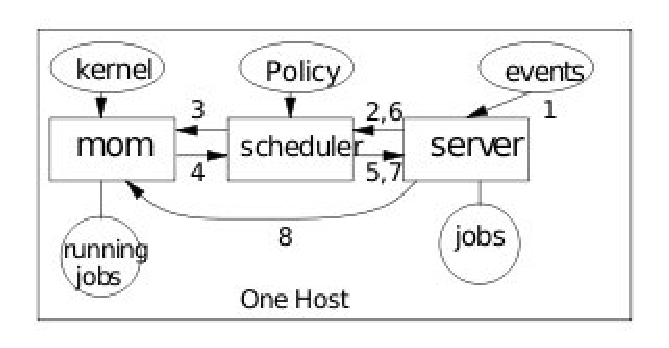
\includegraphics[scale=0.9]{./img/PbsMom.eps}
\caption{Escalonamento em um nó}
\label{fig:Pbs_MOM}
Fonte: \cite{Bayucan1998}
\end{center}
\end{figure}

Um ponto negativo no PBS é o fato deste ter um servidor centralizando, onde uma pane neste nó, afetaria o sistema por inteiro.

Para acesso as funcionalidades que o PBS oferece são fornecidas duas maneiras, um conjunto de \emph{scripts} de linha de comando e uma biblioteca de programação. A biblioteca escrita na linguagem C denominada \emph{Batch Interface Library} (IFL).

O próximo capítulo faz uma análise sobre o modelo GRAND, suas características bem como o protótipo AppMan desenvolvido nos padrões do modelo GRAND.
\chapter{Modelo GRAND}
\label{cap:grand}

No modelo GRAND são tratados três aspectos do gerenciamento de dados: transferência automática dos dados de entrada para o local onde o arquivo será necessário; o envio de resultados é controlado evitando congestionamento da rede; priorização de localidade no disparo de tarefas para não haver transferências desnecessárias de dados degradando o desempenho. Através de uma hierarquia de gerenciadores (Figura 1) é feito o disparo e controle das aplicações. o \emph{Application Manager} (AP) recebe uma submissão de aplicação através de um usuário, os APs mandam os \emph{Submission Managers} (SM) descrições de tarefas assim, sob demanda, são instanciados os \emph{Task Managers} (TM) para controlar a submissão de tarefas a escalonadores de domínios específicos da grade, esses escalonadores recebem requisições dos TMs fazendo a execução das tarefas propriamente ditas.

Pelo fato de que, na atualidade, ambientes grades envolvem principalmente instituições de ensino em aplicações usualmente classificadas como aplicações científicas, o escopo do GRAND é limitado as seguintes itens. 

\begin{enumerate}
    \item heterogeneidade, lembrando que isto afeta diretamente a política de escalonamento por necessitar de saber as características distintas de hardware e software; 
    \item grande número de submissão de tarefas, referindo-se a aplicações que geram centenas ou milhares de processos; 
    \item ausência de comunicação por troca de mensagens, pelo fato da necessidade de inúmeros aspectos nas fases de agrupamento e mapeamento serem considerados; 
    \item interdependência de tarefas, devido ao compartilhamento de arquivos; 
    \item manipulação de grande número de arquivos pelas tarefas; 
    \item o uso de arquivos grandes, através de técnicas como \emph{staging} e \emph{caching}, minimizando a perda de desempenho em função da latência de transmissão; 
    \item segurança, assume-se que exista uma conexão segura entre os nós da grade; 
    \item descoberta dinâmica de recursos; 
    \item gerenciador de recursos local em cada nó; 
    \item uma tarefa é executada em um RMS até sua finalização;
\end{enumerate}

\begin{figure}[htb]
\begin{center}
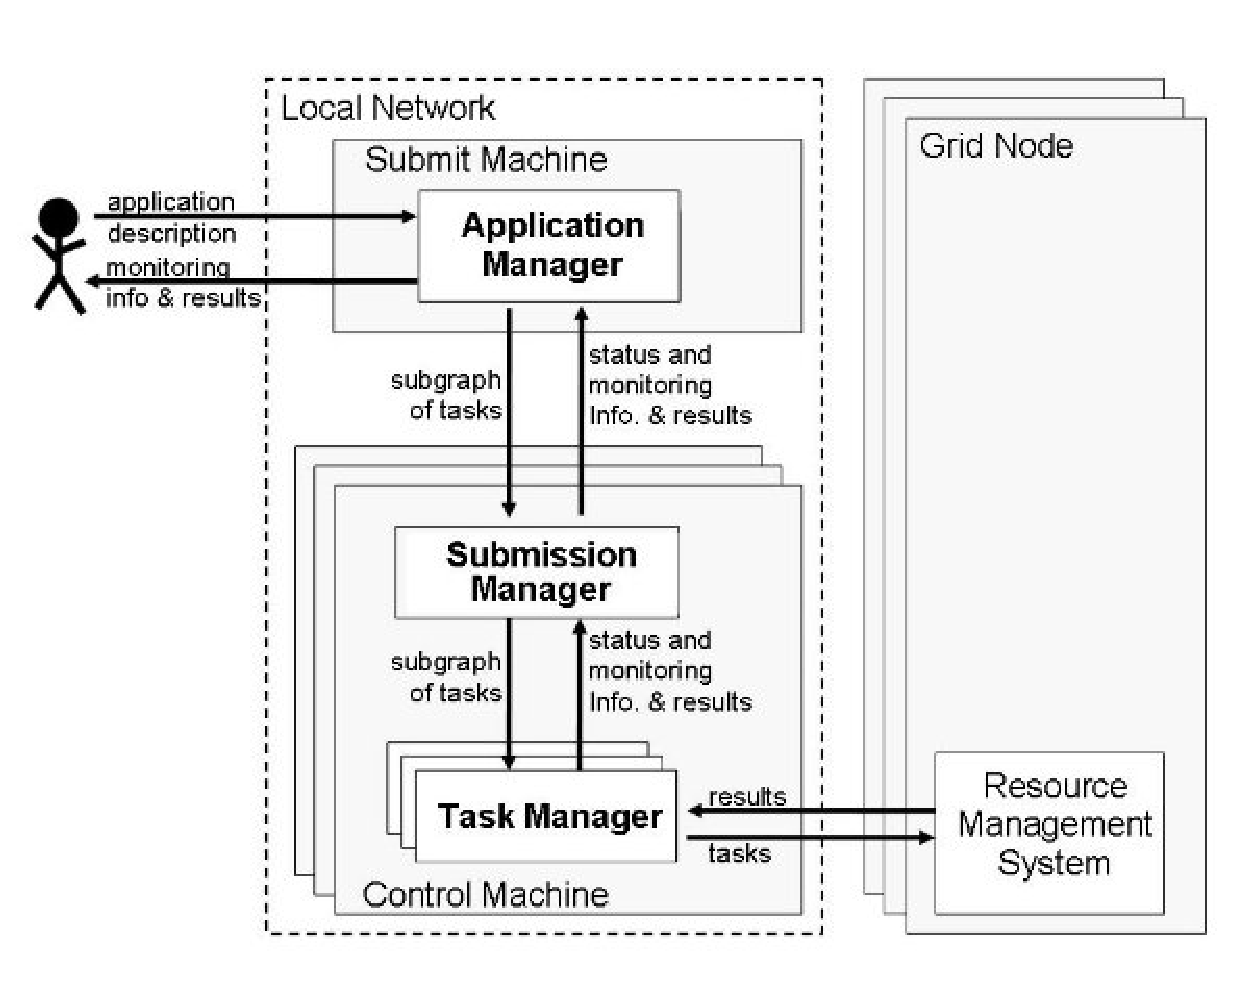
\includegraphics[scale=0.7]{./img/grand.eps}
\caption{Principais componentes do modelo hierárquico de gerenciamento de tarefas}
\label{fig:Modelo_Grand}
\end{center}
\end{figure}

\section{Característica das Aplicações}

Baseando-se em aplicações típicas para ambientes de grades, comunicando-se via troca de arquivo, conhecimento do número de processo a serem criados e sem troca de mensagens, é proposta a seguinte taxonomia de aplicações \emph{ver as bibliografias que consta na página 23 da tese da kayser}

\begin{itemize}
	\item tarefas independentes \emph{\textbf{independent tasks}} ou seja, as tarefas não possuem dependência entre si. Muitas vezes chamado de \emph{bag-of-tasks}.
	\item tarefas fracamente acopladas \emph{\textbf{loosely-coupled tasks}} tarefas com poucos pontos de compartilhamentos, aplicações dividas em fases ou sequência.
	\item tarefas fortemente acopladas \emph{\textbf{tightly-coupled tasks}} grafos complexos, aplicações em lógica com restrições.
\end{itemize}

\begin{figure}[htb]
\begin{center}
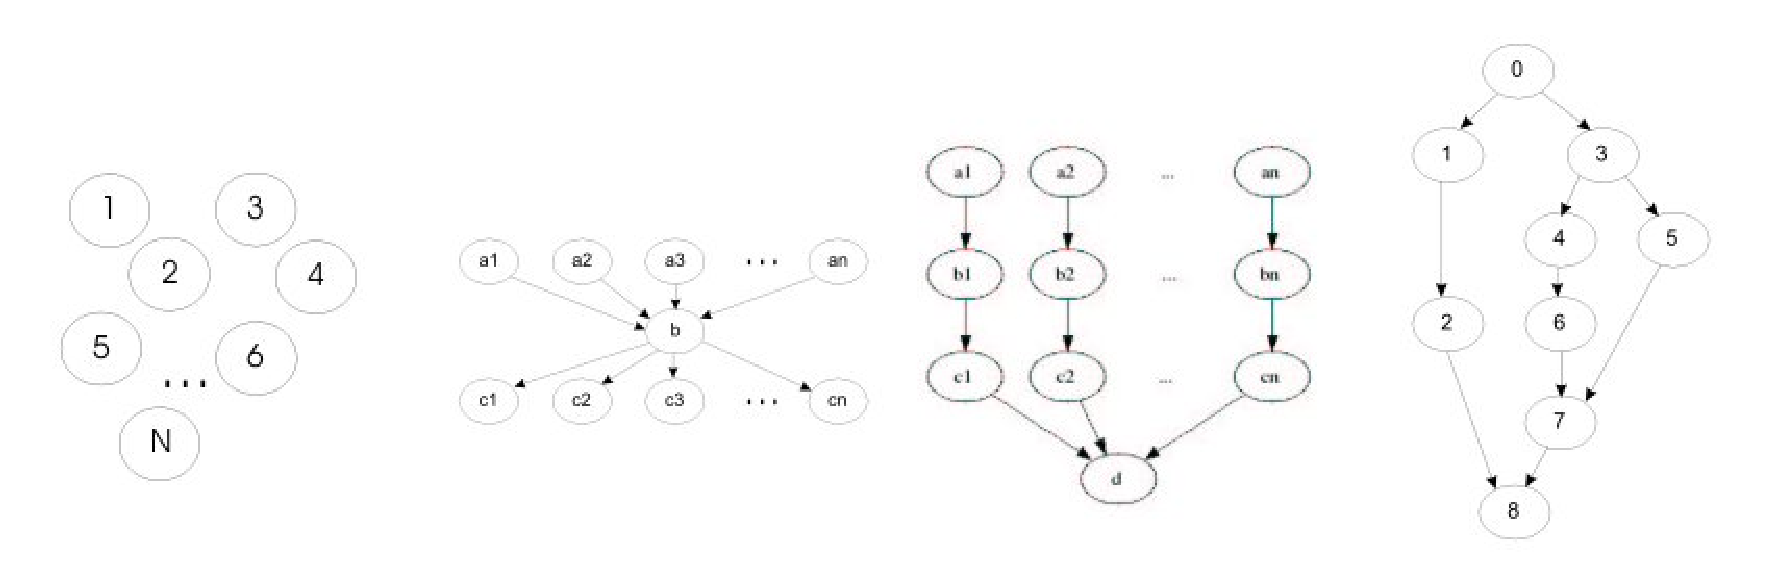
\includegraphics[scale=0.5]{./img/TaxonomiaAplicacoes.eps}
\caption{Categorias de aplicações de grade: (a) \emph{independent tasks}, (b) \emph{loosely-coupled task(phase)}, (c) \emph{loosely-coupled tasks (pipeline)} e (d) \emph{tightly-coupled tasks}}
\label{fig:Taxonomia_Aplicacoes}
\end{center}
\end{figure}

\section{Gerenciamento de Dados}

Ainda há muito o que ser feito nesta questão, até então o tratamento dos dados é resolvido através de soluções distintas. A preocupação principal de vários trabalhos \emph{CITAR GLOBUS E GRIDFTP} é com dados em forma de arquivos.

No GRAND, o gerenciamento de arquivos é apenas com \emph{stage in} e \emph{stage out}, ou seja, enviar os dados para o local de processamento e retorno de resultados. 


\section{Particionamento}

\section{Modelo de Gerenciamento}

    %\section{Gerenciamento de Recursos}

Devido à grande escala, ampla distribuição e existência de múltiplos domínios administrativos, a construção de um escalonador central de recursos para grades é praticamente inviável, até porque, convencer os administradores dos recursos que compõem a grade abrirem mão do controle dos seus recursos não é uma tarefa nada fácil. Escalonadores têm como características receber solicitações de vários usuários, arbitrando, portanto, entre os usuários, o uso dos recursos controlados.  

Casavant \cite{Thomas1996} considera escalonar como um problema de gerenciamento de recursos. Basicamente, escalonador é um mecanismo ou uma política usada para, eficientemente e efetivamente, gerenciar o acesso e uso de um determinado recurso. De acordo com o OGF's \cite{M.2002}, escalonamento é o processo de ordenar tarefas sobre os recursos computacionais e ordenar a comunicação entre as tarefas, assim sendo, ambas aplicações e sistemas devem ser escalonadas. 

O gerenciamento de recursos de um sistema centralizado possui informação completa e atualizada do estado (\emph{status}) dos recursos gerenciados. Este difere do sistema distribuído, o qual não tem conhecimento global de recursos dificultando assim, o gerenciamento. O ambiente em grade introduz cinco desafios para o problema de gerenciamento de recursos em ambientes distribuídos \cite{Karl1998}:

\begin{enumerate}
\item autonomia: os recursos são, tipicamente propriedades e operados por diferentes organizações em diferentes domínios administrativos;
\item heterogeneidade: diferentes lugares podem usar diferentes sistemas de gerenciamento de recursos (RMS);
\item extender as políticas: suporte no desenvolvimento de nova aplicação de mecanismos de gerência num domínio específico, sem necessitar de mudanças no código instalado nos domínios participantes;
\item co-alocação: algumas aplicações tem necessidades de recursos os quais só podem ser satisfeitos apenas usando recursos simultâneos com vários domínios;
\item controle online: RMSs precisam suportar negociações para adaptar necessidades de aplicações para recursos disponíveis.
\end{enumerate}

Sistemas computacionais, em muitos casos, falham ao tratar dois problemas \cite{Mangan2006}: 

\begin{itemize}
	\item gerenciamento e controle de um grande número de tarefas; 
	\item o balanceamento da carga da máquina de submissão e do tráfego da rede.
\end{itemize}

Uma distribuição dinâmica de dados e tarefas em uma hierarquia de gerenciadores poderia ajudar o gerenciamento de aplicações. O modelo GRAND baseado na submissão e controle particionados e hierárquicos foi detalhado em \cite{Mangan2006}. Uma explanação mais detalhada deste modelo será dada no próximo capítulo.

Grande parte das pesquisas sobre escalonamento de tarefas em grades seguem uma organização hierárquica ou centralizada tais como: Globus \cite{Foster1998}, Condor \cite{condor2007}, ISAM \cite{isam} e PBS \cite{Bayucan1998}.

Globus \cite{Globus}, um dos projetos mais referenciados na literatura, tem como principal software o Globus Toolkit (GT). Como o nome indica, o GT não é uma solução completa e sim um conjunto de serviços que podem ser combinados para a construção de um \emph{middleware} de grade. O Globus \cite{Foster1998} tem seu modelo de escalonamento centralizado. Não fornece suporte nativo as políticas de escalonamento mas permite que gerenciadores externos adicionem esta capacidade. O Globus (GT versão 3) oferece serviços de informação através de uma rede hierárquica chamada \emph{Metacomputing Directory Services} (MDS) \cite{Santos}. O gerenciamento de cada recurso é feito por uma instância do {\it Globus Resource Allocation Manager} (GRAM) \cite{Andrade2002}. GRAM é o responsável por instanciar, monitorar e reportar o estado das tarefas alocadas para o recurso. A GT4 \cite{Leon2006} disponibiliza tais serviços em uma arquitetura baseada em {\it Web Services} a {\it Open Grid Services Architecture} (OGSA) junto com {\it Web Services Resource Framework} (WSRF). A GT4 é focada na qualidade, robustez, facilidade de uso e documentação.

Outro projeto bastante importante é o Condor \cite{condor2007}, cujos trabalhos originais são voltados para redes de computadores, mas atualmente também contemplam {\it clusters} e grades. O Condor trabalha com a descoberta de recursos ociosos dentro de uma rede alocando esses recursos para execução das tarefas. Condor possui uma arquitetura de escalonamento centralizado, ou seja, uma máquina especial é responsável pelo escalonamento. Todas as máquinas podem submeter tarefas a máquina central que se responsabiliza de encontrar recursos disponíveis para execução da tarefa. Tanto o Condor quanto o Globus perdem pontos no quesito tolerância a falhas e escalabilidade devido ao fato de terem um controle centralizado onde um problema na máquina central comprometeria o sistema por inteiro. Além disso, para o Globus, são necessárias negociações com os donos de recursos além da necessidade do mapeamento dos clientes para usuários locais. O Condor permite interligar redes, desde que configurado manualmente para comunicar os escalonadores.

Já o projeto ISAM \cite{isam} possui uma arquitetura organizada na forma de células autônomas cooperativas. Sua proposta é fornecer uma infra-estrutura tanto para a construção quanto execução de aplicações pervasivas \cite {isam}. Concebida para habilitar as aplicações a obter informações do ambiente onde executam e se adaptam às alterações que ocorrem durante o transcurso da execução. O ISAM, diferente do Globus e do Condor, possui um modelo de escalonador de tarefas descentralizado ajudando o sistema a alcançar um bom nível de tolerância a falhas e escalabilidade.

Um dos gerenciadores que podem ser integrados com o Globus é o PBS \cite{Bayucan1998}. O PBS é um RMS que tem por propósito prover controle adicionais sobre a execução de tarefas em batch. O sistema permite um domínio definir e implementar políticas tais como os tipos de recursos e como esses recursos podem ser usados por diferentes tarefas.

\section{Portable Batch System - PBS}
%\label{cap:pbs}

Desenvolvido para fornecer processamento em lote, ao contrário de colocar um processo em segundo plano, o processamento em lote do PBS abrange o escalonamento de múltiplas tarefas conforme as políticas do RMS. Cada tarefa pode conter inúmeros processos. Essas tarefas podem ser direcionadas para rotear processos através de nós em uma rede. É possível a reserva de recursos para determinada tarefa antes do início da sua execução \cite{Bayucan1998a}.

\section{PBS - Cliente}

Comandos devem estar de acordo com a especificação POSIX.15. É possível especificar mais de uma operação na linha de comando onde essas serão interpretadas uma de cada vez. A geração de um erro de operando em determinado servidor será colocado na saída de erro padrão. O comando continua executando demais operandos. Sendo que o recebimento de qualquer erro por qualquer operando, resultará em um \emph{status} final maior que zero.

\section{PBS - Servidor}

O servidor principal tem como foco principal a comunicação dos clientes e gerenciar as tarefas. O servidor é o coração do sistema e suas principais responsabilidades são \cite{Bayucan1998a}:

\begin{itemize}
	\item possuir e controlar tarefas em lotes.
	\item possuir e controlar filas.
	\item recuperar estado de tarefas e filas.
	\item executar serviços em nome de clientes baseado em um serviço de requisição de lote.
	\item executar serviços adiados em nome de tarefas baseadas em eventos externos.
	\item iniciar seleção de tarefas para execução baseado em um grupo local definido de políticas de regras.
	\item estabelecer recursos reservados e usar limites para tarefas iniciadas no local de execução.
	\item colocar uma tarefa de lote em execução e monitorar seu progresso.
	\item executar o processamento e a limpeza de tarefas.
\end{itemize}

\section{Processo de Escalonamento}

O processo de escalonamento se caracteriza por uma escolha que elege qual tarefa será executada. Para isto, esta tarefa deve constar em uma fila de execução.

O PBS fornece um programa separado como um processo de seleção que maximiza a flexibilidade na implementação das políticas locais. O escalonador comunica-se com o servidor via um \emph{socket} IPC. Desta forma é possível possuir escalonador e servidor em diferentes nós.

Para cumprir seu papel de gerenciador de recursos, o escalonador se comunica com outro processo chamado \emph{Machine Oriented Mineserver} (MOM). Assim é possível recuperar informações sobre a carga do sistema do nó. Nestas informações podem conter detalhes do uso de memória, carga de CPU, entre outras. Esta relação entre PBS, o escalonador e o MOM é demostrado na figura~\ref{fig:Pbs_MOM} \cite{Bayucan1998}.

\begin{center}
	\begin{enumerate}
		\item Evento aviso o servidor para iniciar um ciclo de escalonamento.
		\item Servidor envia comando de escalonamento para Escalonador.
		\item Escalonador requisita informação de recursos do MOM.
		\item MOM retorna informações solicitadas.
		\item Escalonador requisita informações do servidor.
		\item Servidor envia informações de \emph{status} da tarefa para o escalonador. Escalonador realiza política para executar a tarefa.
		\item Escalonador envia solicitação de execução para o servidor.
		\item Servidor envia tarefa para o MOM executar.
	\end{enumerate}
\end{center}

\begin{figure}[htb]
\begin{center}
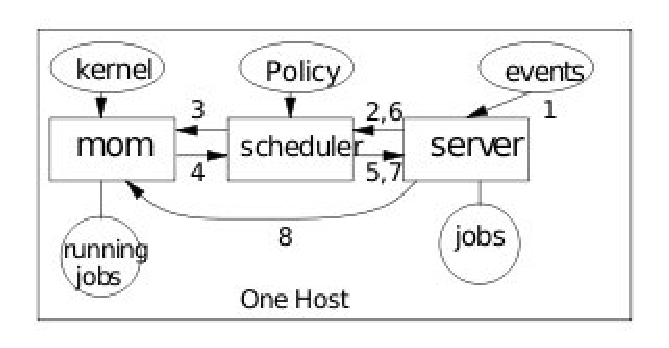
\includegraphics[scale=0.9]{./img/PbsMom.eps}
\caption{Escalonamento em um nó}
\label{fig:Pbs_MOM}
Fonte: \cite{Bayucan1998}
\end{center}
\end{figure}

Um ponto negativo no PBS é o fato deste ter um servidor centralizando, onde uma pane neste nó, afetaria o sistema por inteiro.

Para acesso as funcionalidades que o PBS oferece são fornecidas duas maneiras, um conjunto de \emph{scripts} de linha de comando e uma biblioteca de programação. A biblioteca escrita na linguagem C denominada \emph{Batch Interface Library} (IFL).

O próximo capítulo faz uma análise sobre o modelo GRAND, suas características bem como o protótipo AppMan desenvolvido nos padrões do modelo GRAND.
    \chapter{Modelo GRAND}
\label{cap:grand}

No modelo GRAND são tratados três aspectos do gerenciamento de dados: transferência automática dos dados de entrada para o local onde o arquivo será necessário; o envio de resultados é controlado evitando congestionamento da rede; priorização de localidade no disparo de tarefas para não haver transferências desnecessárias de dados degradando o desempenho. Através de uma hierarquia de gerenciadores (Figura 1) é feito o disparo e controle das aplicações. o \emph{Application Manager} (AP) recebe uma submissão de aplicação através de um usuário, os APs mandam os \emph{Submission Managers} (SM) descrições de tarefas assim, sob demanda, são instanciados os \emph{Task Managers} (TM) para controlar a submissão de tarefas a escalonadores de domínios específicos da grade, esses escalonadores recebem requisições dos TMs fazendo a execução das tarefas propriamente ditas.

Pelo fato de que, na atualidade, ambientes grades envolvem principalmente instituições de ensino em aplicações usualmente classificadas como aplicações científicas, o escopo do GRAND é limitado as seguintes itens. 

\begin{enumerate}
    \item heterogeneidade, lembrando que isto afeta diretamente a política de escalonamento por necessitar de saber as características distintas de hardware e software; 
    \item grande número de submissão de tarefas, referindo-se a aplicações que geram centenas ou milhares de processos; 
    \item ausência de comunicação por troca de mensagens, pelo fato da necessidade de inúmeros aspectos nas fases de agrupamento e mapeamento serem considerados; 
    \item interdependência de tarefas, devido ao compartilhamento de arquivos; 
    \item manipulação de grande número de arquivos pelas tarefas; 
    \item o uso de arquivos grandes, através de técnicas como \emph{staging} e \emph{caching}, minimizando a perda de desempenho em função da latência de transmissão; 
    \item segurança, assume-se que exista uma conexão segura entre os nós da grade; 
    \item descoberta dinâmica de recursos; 
    \item gerenciador de recursos local em cada nó; 
    \item uma tarefa é executada em um RMS até sua finalização;
\end{enumerate}

\begin{figure}[htb]
\begin{center}
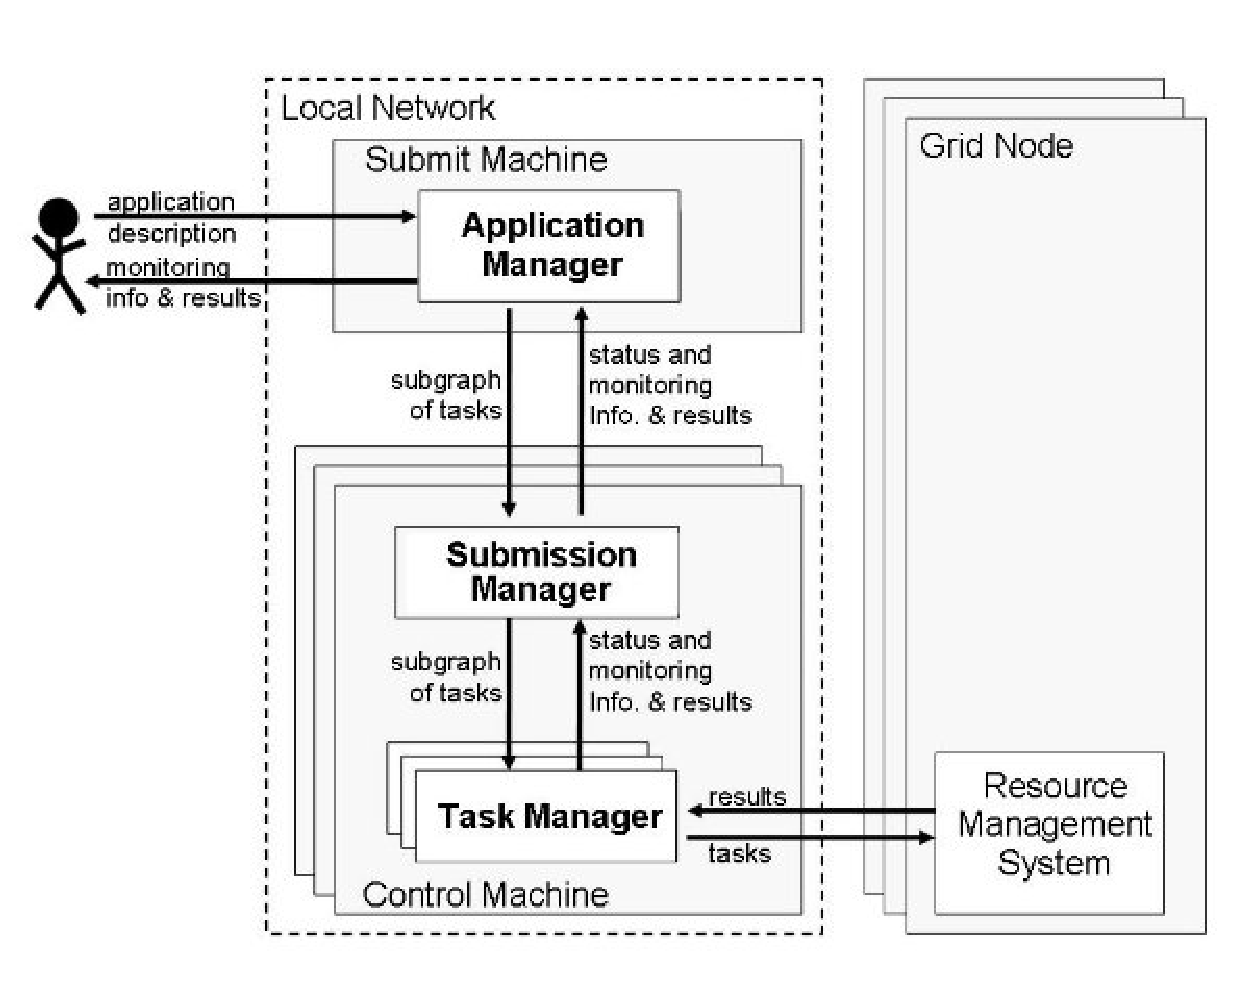
\includegraphics[scale=0.7]{./img/grand.eps}
\caption{Principais componentes do modelo hierárquico de gerenciamento de tarefas}
\label{fig:Modelo_Grand}
\end{center}
\end{figure}

\section{Característica das Aplicações}

Baseando-se em aplicações típicas para ambientes de grades, comunicando-se via troca de arquivo, conhecimento do número de processo a serem criados e sem troca de mensagens, é proposta a seguinte taxonomia de aplicações \emph{ver as bibliografias que consta na página 23 da tese da kayser}

\begin{itemize}
	\item tarefas independentes \emph{\textbf{independent tasks}} ou seja, as tarefas não possuem dependência entre si. Muitas vezes chamado de \emph{bag-of-tasks}.
	\item tarefas fracamente acopladas \emph{\textbf{loosely-coupled tasks}} tarefas com poucos pontos de compartilhamentos, aplicações dividas em fases ou sequência.
	\item tarefas fortemente acopladas \emph{\textbf{tightly-coupled tasks}} grafos complexos, aplicações em lógica com restrições.
\end{itemize}

\begin{figure}[htb]
\begin{center}
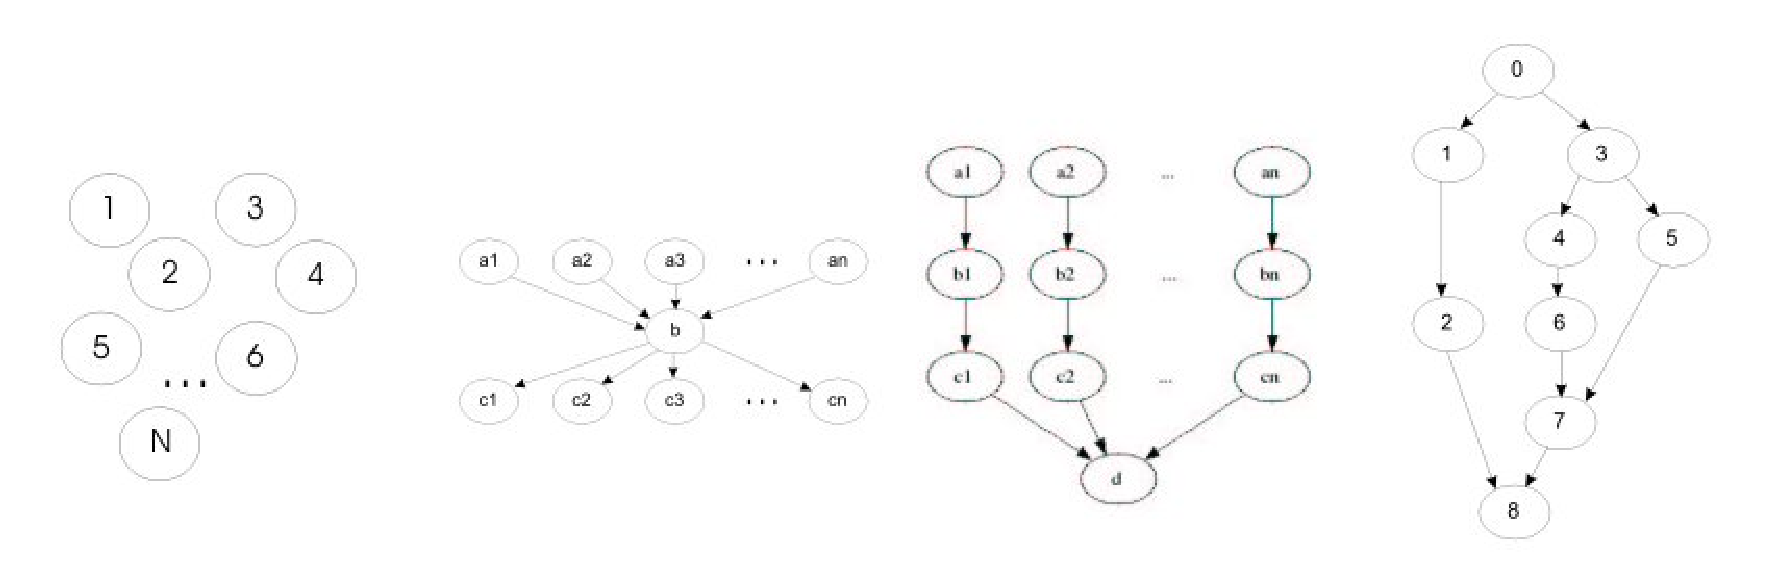
\includegraphics[scale=0.5]{./img/TaxonomiaAplicacoes.eps}
\caption{Categorias de aplicações de grade: (a) \emph{independent tasks}, (b) \emph{loosely-coupled task(phase)}, (c) \emph{loosely-coupled tasks (pipeline)} e (d) \emph{tightly-coupled tasks}}
\label{fig:Taxonomia_Aplicacoes}
\end{center}
\end{figure}

\section{Gerenciamento de Dados}

Ainda há muito o que ser feito nesta questão, até então o tratamento dos dados é resolvido através de soluções distintas. A preocupação principal de vários trabalhos \emph{CITAR GLOBUS E GRIDFTP} é com dados em forma de arquivos.

No GRAND, o gerenciamento de arquivos é apenas com \emph{stage in} e \emph{stage out}, ou seja, enviar os dados para o local de processamento e retorno de resultados. 


\section{Particionamento}

\section{Modelo de Gerenciamento}
    \chapter{A Especificação DRMAA}
\label{cap:drmaa}

\emph{Distributed Resource Management Application API} (DRMAA) abstrai as diferenças dos RMS fornecendo uma API para programadores de aplicações distribuídas. 

O escopo da DRMAA é limitado em submeter, monitorar e controlar as aplicações, recuperando o \emph{status} de término da tarefa.

A idéia é que a API seja implementada em múltiplas linguagens. Implementada inicialmente em C/C++, tendo como segunda opção linguagens de \emph{scripts} tais como \emph{Perl} e \emph{Python}. O desenvolvimento da \emph{Interface Definition Language} (IDL) soluciona o problema através de uma \emph{interface} que serve para múltiplas linguagens.

Uma biblioteca ideal deveria servir, dinâmica e estaticamente, para todos RMS e suas versões. Porém, é possível implementar múltiplos mas não todos RMSs.

A idéia da implementação e aplicações distribuídas em larga escala são para um ambiente DRM e suas políticas. Nem sempre isto é possível, então uma solução menos intrusiva com uma "categoria de tarefa" e "especificação nativa", tem sido proposta. As políticas específicas do lugar são abstraídas/agregadas em simples \emph{strings} que são interpretadas pela implementação DRMAA. DRMAA não possui um mecanismo explícito de organização de arquivos  \cite{Rajic2004}. 

\section{Categorias de Tarefas}

Experiências com integrações em um DRM mostra que mesmo uma aplicação de mesmo \emph{Independent Software Vendor} (ISV) possuem políticas diferenciadas através de usuários. Essas políticas afetam atributos específicos tais como os recursos usados pela tarefa, preferência de localidade da execução da tarefa e onde a tarefa irá ser escalonada com relação a outras tarefas.

DRMAA fornece formas distintas para "\emph{job categories}" que encapsulam detalhes das tarefas específicas, escondendo estes detalhes da aplicação. É possível criar uma categoria de tarefa específica para uma aplicação a ser dispachada pelo DRMS, o nome associado a categoria deve ser especificado como um atributo de submissão de tarefa. A DRMAA pode, então, usar o nome da categoria para gerenciar recursos específicos do local e requisitos funcionais das tarefas.

Um problema típico que dificulta a escrita para muitos ISVs é o não conhecimento prévio da configuração do DRMS, ainda assim a DRMAA facilita a escrita de aplicações \cite{Rajic2002}.

\section{DRMAA para PBS}

A biblioteca cobre aproximadamente toda a especificação DRMAA 1.0 com as exceções listadas \cite{drmaa_pbs}. Ela passou no teste oficial da \emph{suite} DRMAA com excessão dos testes que requerem \emph{status} de término de tarefa. Todos os obrigatórios e alguns atributos opcionais de tarefas são implementados.

\begin{itemize}
	\item com PBS, recuperar o \emph{status} de uma tarefa terminada é impossível. Por isso tarefas terminadas são marcadas como completas com código de retorno 0 desde que não tenham terminadas através da biblioteca.
	\item apenas são aceitas tarefas submetidas sob a sessão corrente (especificação diz que devem ser aceitas tarefas identificadas da sessão anterior).
	\item o estado do término da tarefa, quando realizado pelo PBS, é marcado como "abortado"  e  "marcado" qualquer que seja o estado.
	\item drmaa-wcoredump() sempre retorna \emph{false}.
\end{itemize}

\section{A Java \emph{Binding} API}

Apesar da especificação GFD.022 ter uma tendência para linguagem C, há uma liberdade para melhorar o ajuste com uma linguagem orientada a objetos como o Java. Alguns métodos sugerido na especificação não constam nos \emph{bindings} de linguagens orientadas a objetos. Os métodos drmaa\underline{ }get\underline{ }attribute(), drmaa\underline{ }set\underline{ }attribute(), drmaa\underline{ }get\underline{ }vector\underline{ }attribute(), drmaa\underline{ }set\underline{ }vector\underline{ }attribute() e drmaa\underline{ }get\underline{ }vector\underline{ } attribute \underline{ }names() não são necessários pois a especificação do \emph{binding} Java especifica uma propriedade \emph{\textbf{getter}} e \emph{\textbf{setter}} para cada atributo DRMAA. Um \emph{getter} é um método para recuperar valores e um método \emph{setter} para atribuir valores. Essas propriedades permitem, em tempo de compilação, chechar os atributos DRMAA permitindo especial tratamento dos atributos que são melhores representados como algo diferente de uma \emph{String} \cite{Templeton2003}.

No capítulo seguinte é feito uma análise do PBS, RMS usado na integração com o protótipo AppMan.
    %\section{Portable Batch System - PBS}
%\label{cap:pbs}

Desenvolvido para fornecer processamento em lote, ao contrário de colocar um processo em segundo plano, o processamento em lote do PBS abrange o escalonamento de múltiplas tarefas conforme as políticas do RMS. Cada tarefa pode conter inúmeros processos. Essas tarefas podem ser direcionadas para rotear processos através de nós em uma rede. É possível a reserva de recursos para determinada tarefa antes do início da sua execução \cite{Bayucan1998a}.

\section{PBS - Cliente}

Comandos devem estar de acordo com a especificação POSIX.15. É possível especificar mais de uma operação na linha de comando onde essas serão interpretadas uma de cada vez. A geração de um erro de operando em determinado servidor será colocado na saída de erro padrão. O comando continua executando demais operandos. Sendo que o recebimento de qualquer erro por qualquer operando, resultará em um \emph{status} final maior que zero.

\section{PBS - Servidor}

O servidor principal tem como foco principal a comunicação dos clientes e gerenciar as tarefas. O servidor é o coração do sistema e suas principais responsabilidades são \cite{Bayucan1998a}:

\begin{itemize}
	\item possuir e controlar tarefas em lotes.
	\item possuir e controlar filas.
	\item recuperar estado de tarefas e filas.
	\item executar serviços em nome de clientes baseado em um serviço de requisição de lote.
	\item executar serviços adiados em nome de tarefas baseadas em eventos externos.
	\item iniciar seleção de tarefas para execução baseado em um grupo local definido de políticas de regras.
	\item estabelecer recursos reservados e usar limites para tarefas iniciadas no local de execução.
	\item colocar uma tarefa de lote em execução e monitorar seu progresso.
	\item executar o processamento e a limpeza de tarefas.
\end{itemize}

\section{Processo de Escalonamento}

O processo de escalonamento se caracteriza por uma escolha que elege qual tarefa será executada. Para isto, esta tarefa deve constar em uma fila de execução.

O PBS fornece um programa separado como um processo de seleção que maximiza a flexibilidade na implementação das políticas locais. O escalonador comunica-se com o servidor via um \emph{socket} IPC. Desta forma é possível possuir escalonador e servidor em diferentes nós.

Para cumprir seu papel de gerenciador de recursos, o escalonador se comunica com outro processo chamado \emph{Machine Oriented Mineserver} (MOM). Assim é possível recuperar informações sobre a carga do sistema do nó. Nestas informações podem conter detalhes do uso de memória, carga de CPU, entre outras. Esta relação entre PBS, o escalonador e o MOM é demostrado na figura~\ref{fig:Pbs_MOM} \cite{Bayucan1998}.

\begin{center}
	\begin{enumerate}
		\item Evento aviso o servidor para iniciar um ciclo de escalonamento.
		\item Servidor envia comando de escalonamento para Escalonador.
		\item Escalonador requisita informação de recursos do MOM.
		\item MOM retorna informações solicitadas.
		\item Escalonador requisita informações do servidor.
		\item Servidor envia informações de \emph{status} da tarefa para o escalonador. Escalonador realiza política para executar a tarefa.
		\item Escalonador envia solicitação de execução para o servidor.
		\item Servidor envia tarefa para o MOM executar.
	\end{enumerate}
\end{center}

\begin{figure}[htb]
\begin{center}
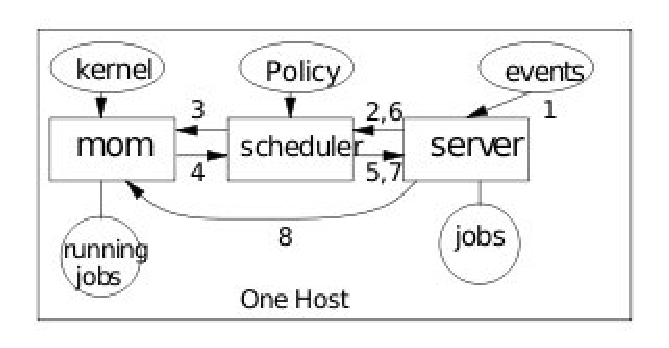
\includegraphics[scale=0.9]{./img/PbsMom.eps}
\caption{Escalonamento em um nó}
\label{fig:Pbs_MOM}
Fonte: \cite{Bayucan1998}
\end{center}
\end{figure}

Um ponto negativo no PBS é o fato deste ter um servidor centralizando, onde uma pane neste nó, afetaria o sistema por inteiro.

Para acesso as funcionalidades que o PBS oferece são fornecidas duas maneiras, um conjunto de \emph{scripts} de linha de comando e uma biblioteca de programação. A biblioteca escrita na linguagem C denominada \emph{Batch Interface Library} (IFL).
    \chapter{Integração do AppMan com a especificação DRMAA}
\label{cap:implementacao}

O protótipo AppMan ainda está em desenvolvimento, portanto nem todos os requisitos descritos no modelo GRAND constam no protótipo e, seu funcionamento ainda apresenta alguns comportamentos inesperados. 

Desenvolvido com seu código fonte aberto, seus fontes estão em um repositório acessível para qualquer um que deseja visualizá-los.

Este trabalho foi desenvolvido usando como base arquivos existente em um \emph{branch} do repositório svn que o AppMan se encontra. De acordo com a documentação contida nestes arquivos, eles já possuem uma integração através do uso da DRMAA. Ao testar esses arquivos esta versão não estava funcional. Alguns ajustes, que serão explicados posteriormente, foram necessários para o funcionamento correto desta versão.

\section{Criação do Ambiente Computacional}

Para o desenvolvimento do trabalho proposto foi criado um ambiente computacional com um RMS OpenPBS instalado possuindo três nós para submissão de tarefas. Foi configurado um servidor LDAP necessário para a execução do middleware EXEHDA/ISAM. A instalação do OpenPBS foi feito em um computador com processador AMD Turion(tm) 64 X2 Mobile Technology TL-50 1.6Ghz e 1.5Gb de memória RAM. O Servidor LDAP foi instalando em um computador AMD Athlon(tm) 64 X2 Dual Core Processor 4000+ 2.2Ghz e memório RAM de 2.0Gb. Este computador também está na lista de nós do OpenPBS além de mais dois outros. O primeiro possui processador AMD Sempron(tm) 2500+ 1.8Ghz e memória RAM de 512Mb e o outro possui um processador Intel(R) Celeron(R) 2.00GHz com 512Mb de memória RAM. Em todos os computadores o sistema operacional é Linux Ubuntu 7.10 com Kernel 2.6.22.

Para compilação e alterações nos fontes do protótipo foi usado as IDEs NetBeans\cite{netbeans} e Eclipse\cite{eclipse}, para geração de diagramas UML bem como a engenharia reversa do AppMan, foi usado, além das IDEs citadas, o software Umbrello\cite{umbrello}.

\section{Componente DRMAA (submissão e monitoração)}

Baseado na implementação desenvolveu-se um modelo definido por um conjunto de classes conforme figura 6.1. Os principais métodos necessários para submissão e monitoração de uma tarefa estão na classe \emph{appman.rmswrapper.pbs.drmaa.SessionImpl} que implementa a \emph{interface} \emph{org.ggf.drmaa.Session}.

A DRMAA java \emph{binding} foi implementada com a JAVA \emph{Native Interface} (JNI). JNI é uma \emph{interface} de padrão de programação para escrever métodos Java sob uma máquina virtual Java (JVM), fazendo chamadas recebendo chamadas de aplicações nativas. Essas aplicações nativas, são aplicações específicas do sistema operacional. Dentre as linguagens, pode-se fazer chamadas em C++, C e \emph{Assembly} \cite{jni}.

\begin{figure}[htb]
\begin{center}
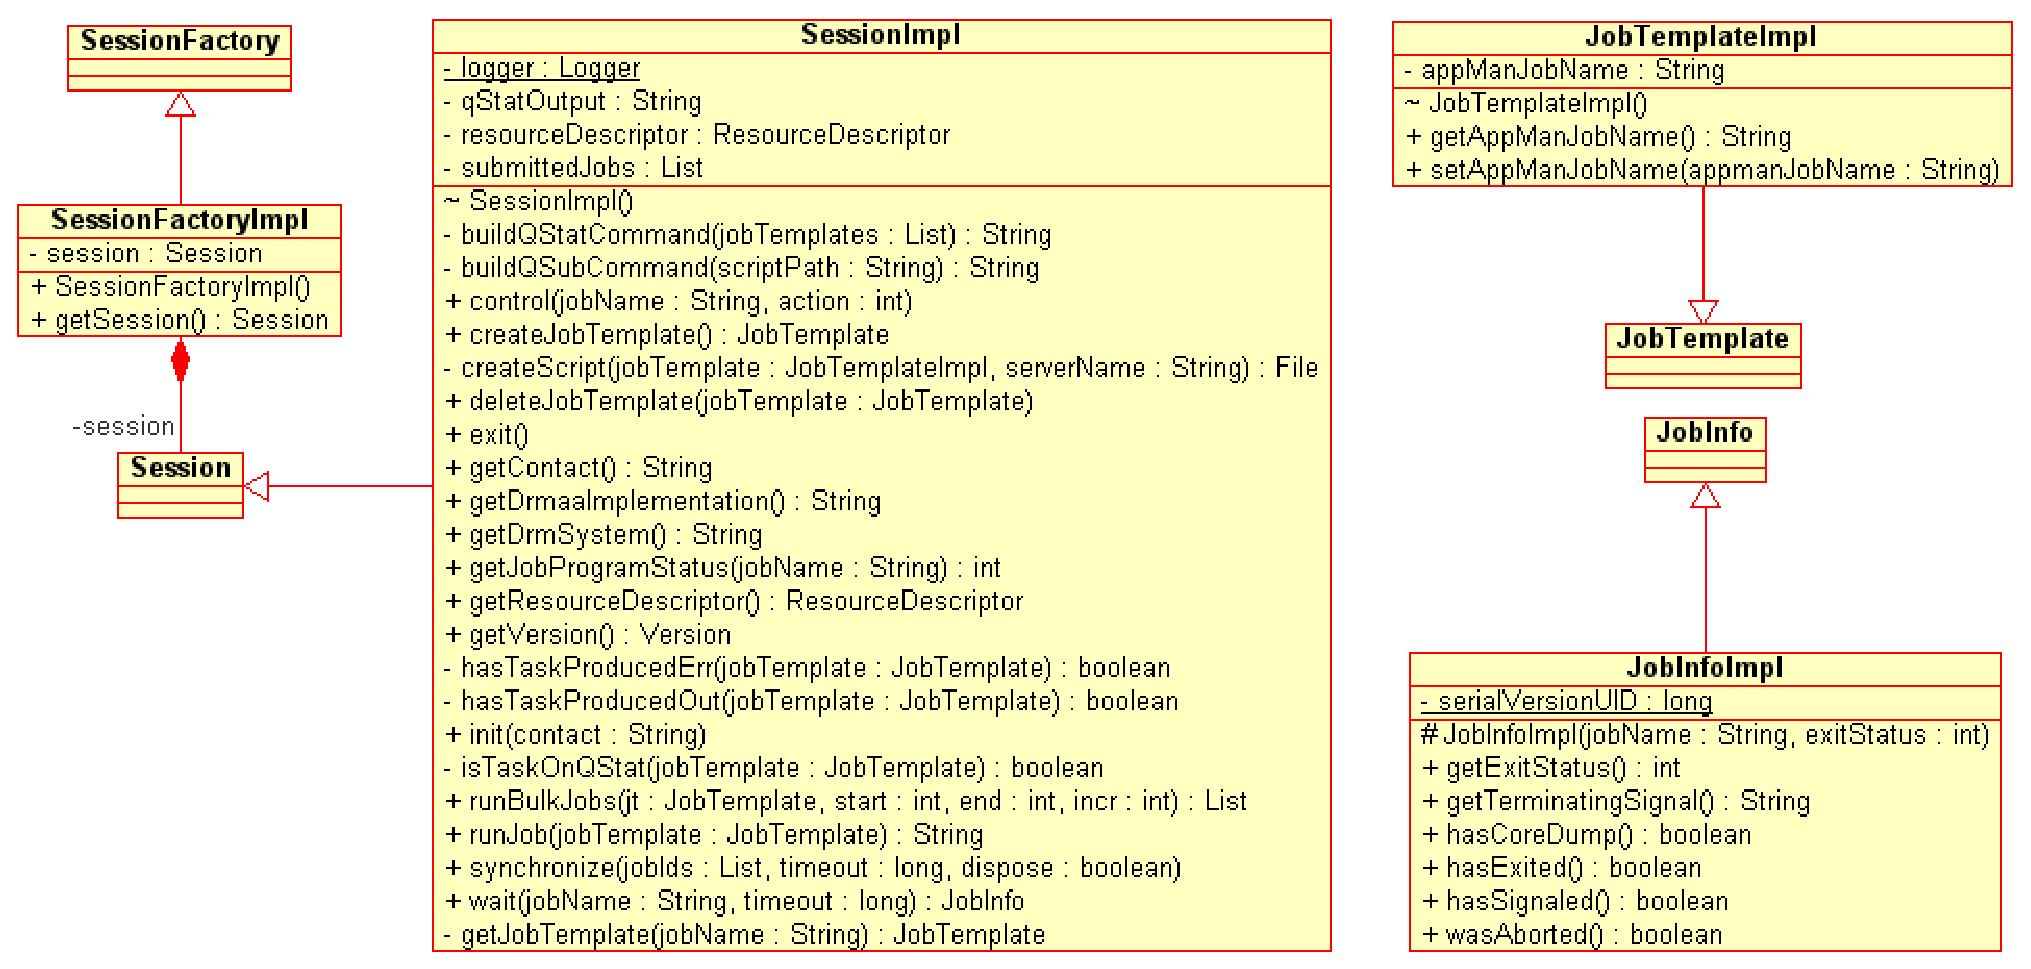
\includegraphics[scale=0.5]{./img/drmaaUML2.eps}
\caption{Diagrama de classes do pacote \textbf{appman.rmswrapper.pbs.drmaa}}
\label{fig:UML_DRMAA}
\end{center}
\end{figure}

Dentre os inúmeros métodos existentes na classe \emph{SessionImpl} os mais relevantes para o AppMan são:

\begin{itemize}
	\item \emph{String runJob(JobTemplate jobTemplate)} submete uma tarefa e tem como retorno um identificador para ser usado se necessário.
	\item \emph{JobInfo wait(String jobName, long timeout)} espera o final da execução por um determinado tempo máximo.
	\item \emph{appman.rmswrapper.pbs.drmaa.JobTemplateImpl} encapsula a definição de uma tarefa para submissão.
	\item \emph{appman.rmswrapper.pbs.drmaa.JobInfoImp} representa a tarefa após a sua execução.
\end{itemize}

\section{AppMan com DRMAA}

Conforme análise do código encontrado no repositório, a integração ficou concentrada em duas mudanças. A primeira é a criação de uma classe nova \emph{appman.GridTaskDrmaa} e a outra foi uma alteração no arquivo de configuração que indica em qual componente é responsável para executação da tarefa, ou \emph{middleware} EXEHDA, ou nova implementação. Com isso, o impacto da modificação torna-se relativamente baixo. 

\subsection{Classe GridTaskDrmaa}

A nova classe implementa a mesma \emph{interface} que a classe padrão \emph{appman.GridTask}. A maior alteração encontra-se no método \emph{execute} onde são feitas as chamadas ao componente de submissão. O método \emph{execute} figura 6.2, é onde são realizados os passos indicados pela especificação DRMAA na submissão e monitoração de tarefas.

\begin{figure}[htb]
\begin{center}
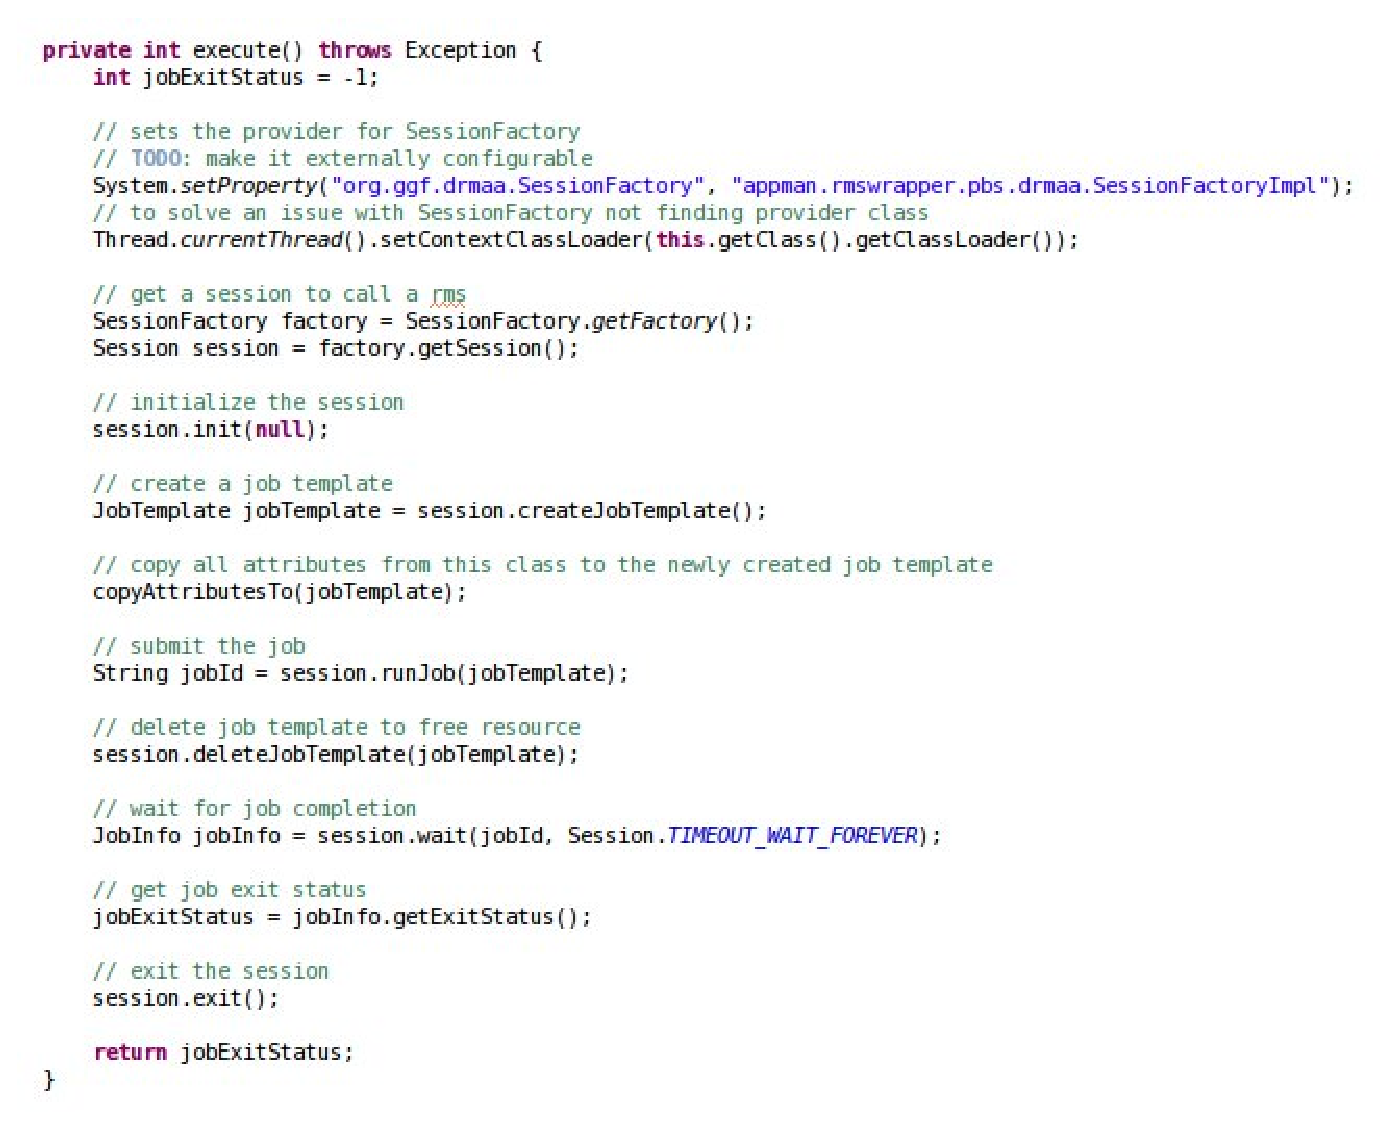
\includegraphics[scale=0.65]{./img/execute.eps}
\caption{Método \emph{execute} da nova classe \emph{appman.GridTaskDrmaa}}
\label{fig:UML_DRMAA}
\end{center}
\end{figure}

\subsection{Arquivo de configuração}

A alteração no arquivo de configuração foi feita para que o nó saiba que componente usar na submissão da tarefa. Esta alteração consiste na criação de uma propriedade que recebe o valor que indica qual componente usar. A figura x exemplifica o arquivo de configuração onde o \emph{Submission Manager} criado no nó \textbf{0.desktop} usará a \emph{GridTaskDrmaa} para submeter tarefas e o nó \textbf{0.notebook} usará \emph{GridTask} para submeter.

\begin{figure}[htb]
\begin{center}
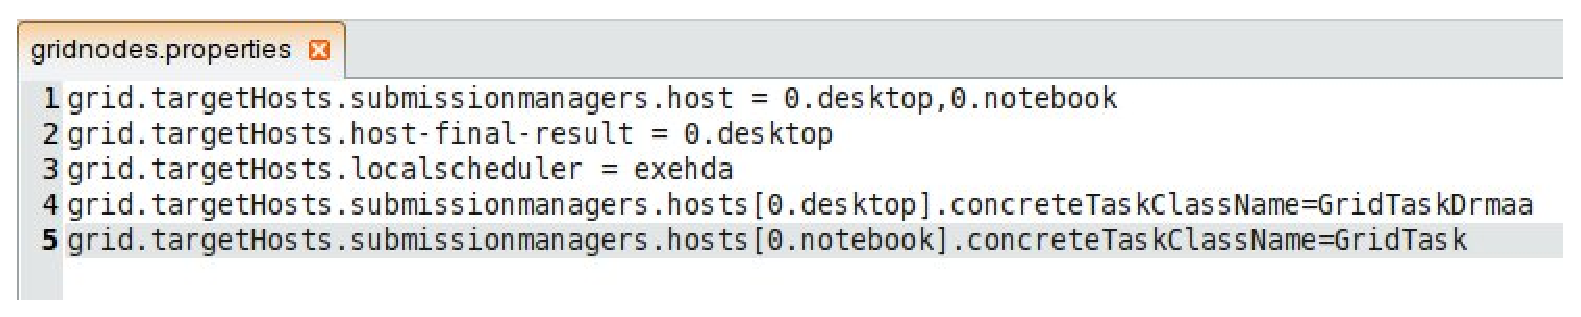
\includegraphics[scale=0.5]{./img/gridnodes_properties.eps}
\caption{Arquivo de configuração \emph{gridnodes.properties}}
\label{fig:gridonodes_properties}
\end{center}
\end{figure}

Para que esta nova configuração fosse reconhecida foi criado o metódo \emph{loadConcreteTaskClassName} na classe \emph{TaskManager} (\textbf{vou colocar uma figura do método}) o qual lê a propriedade no arquivo de configuração e retorna o nome do componente configurado para onde submeter a tarefa. Na implementação atual não foi possível, conforme sugerido, a criação de um \emph{Submission Manager} que submete tarefas via componente DRMAA e um \emph{Submission Manager} usando o componente padrão ao mesmo tempo.
    \bibliographystyle{ieeetr}
\bibliography{biblio}

	 \appendix
\addcontentsline{toc}{chapter}{Apêndices}
\chapter{Arquivo exehda-services.xml de configuração do EXEHDA (sem PBS)}
\label{anexo:exehda-services}

\begin{scriptsize}
\begin{verbatim}
<EXEHDA>

    <PROFILE name="base">

    <PROP name="localhost.id" value="0"/>
    <PROP name="localhost.cell" value="home"/>

    <SERVICE name="logger" loadPolicy="boot">
       <PROP name="impl" value="org.isam.exehda.services.logging.BasicLogger"/>
       <PROP name="logLevel" value="2000"/>
    </SERVICE>

    <SERVICE name="worb" loadPolicy="boot">
       <PROP name="impl" value="org.isam.exehda.services.worb.WorbImpl"/>
    </SERVICE>

    <SERVICE name="cib" loadPolicy="boot">
       <PROP name="impl" value="org.isam.exehda.services.cib.CibImpl"/>
       <PROP name="neighborhood" value="worb:tcp://neo:1980/cib"/>
       <PROP name="backEnd.impl" value="org.isam.exehda.services.cib.backend.ldap.LdapBackEnd"/>
       <PROP name="backEnd.ldap.server" value="neo"/>
       <PROP name="backEnd.ldap.rootDn" value="dc=exehda"/>
       <PROP name="backEnd.ldap.user" value="cn=admin,dc=exehda"/>
       <PROP name="backEnd.ldap.passwd" value="tonismar"/>
    </SERVICE>

    <SERVICE name="bda" loadPolicy="boot">
       <PROP name="impl" value="org.isam.exehda.services.bda.BdaImpl"/>
       <PROP name="docroot" value="/home/tonismar/Publico/appman/lib"/>
    </SERVICE>

    <SERVICE name="avu" loadPolicy="demand">
       <PROP name="impl" value="org.isam.exehda.services.avu.AvuImpl"/>
       <PROP name="docroot" value="/path/to/avu/docroot"/>
    </SERVICE>

   <SERVICE name="executor" loadPolicy="boot">
       <PROP name="impl" value="org.isam.exehda.services.primos.exec.ExecutorImpl"/>
       <PROP name="defaultHeuristic" value="org.isam.exehda.services.primos.exec.HostIdSchedHeuristic"/>
    </SERVICE>

   <SERVICE name="objectseed" loadPolicy="boot">
       <PROP name="impl" value="org.isam.exehda.services.primos.objseed.ObjectSeedImpl"/>
       <PROP name="schedHeuristic" value=""/>
    </SERVICE>

    <SERVICE name="collector" loadPolicy="boot">
       <PROP name="impl" value="org.isam.exehda.services.primos.CollectorImplCell"/>
    </SERVICE>

    <SERVICE name="gatekeeper" loadPolicy="boot">
       <PROP name="impl" value="org.isam.exehda.services.GatekeeperService"/>
       <PROP name="port" value="29901"/>
    </SERVICE>

    <SERVICE name="oxmanager" loadPolicy="boot">
       <PROP name="impl" value="org.isam.exehda.services.oxm.DualOXManagerCell"/>
    </SERVICE>

    <SERVICE name="discoverer" loadPolicy="demand">
       <PROP name="impl" value="org.isam.exehda.services.discoverer.DiscovererImpl"/>
       <PROP name="contactAddress" value="worb:tcp://neo:1980/discoverer" />
    </SERVICE>

  </PROFILE>
    
  <PROFILE name="nodo1">

    <PROP name="localhost.id" value="1"/>
    <PROP name="localhost.cell" value="home"/>
    <SERVICE name="logger" loadPolicy="boot">
       <PROP name="impl" value="org.isam.exehda.services.logging.BasicLogger"/>
       <PROP name="logLevel" value="2000"/>
    </SERVICE>
    <SERVICE name="worb" loadPolicy="boot">
       <PROP name="impl" value="org.isam.exehda.services.worb.WorbImpl"/>
    </SERVICE>
    <SERVICE name="cib" loadPolicy="boot">
       <PROP name="impl" value="org.isam.exehda.services.cib.CibImplClient"/>
       <PROP name="contactAddress" value="worb:tcp://neo:1980/cib"/>
    </SERVICE>
    <SERVICE name="bda" loadPolicy="boot">
       <PROP name="impl" value="org.isam.exehda.services.bda.BdaImplClient"/>
       <PROP name="bdaHost" value="neo" />
    </SERVICE>
    <SERVICE name="executor" loadPolicy="boot">
       <PROP name="impl" value="org.isam.exehda.services.primos.exec.ExecutorImpl"/>
    </SERVICE>
   <SERVICE name="oxmanager" loadPolicy="boot">
       <PROP name="impl" value="org.isam.exehda.services.oxm.OXManagerNode"/>
    </SERVICE>
    <SERVICE name="gatekeeper" loadPolicy="boot">
       <PROP name="impl" value="org.isam.exehda.services.GatekeeperService"/>
    </SERVICE>
    <SERVICE name="objectseed" loadPolicy="boot">
       <PROP name="impl" value="org.isam.exehda.services.primos.objseed.ObjectSeedImpl"/>
    </SERVICE>
    <SERVICE name="collector" loadPolicy="demand">
       <PROP name="impl" value="org.isam.exehda.services.primos.CollectorImplNode"/>
    </SERVICE>
  </PROFILE>

  <PROFILE name="nodo2">

    <PROP name="localhost.id" value="2"/>
    <PROP name="localhost.cell" value="home"/>
    <SERVICE name="logger" loadPolicy="boot">
       <PROP name="impl" value="org.isam.exehda.services.logging.BasicLogger"/>
       <PROP name="logLevel" value="2000"/>
    </SERVICE>
    <SERVICE name="worb" loadPolicy="boot">
       <PROP name="impl" value="org.isam.exehda.services.worb.WorbImpl"/>
    </SERVICE>
    <SERVICE name="cib" loadPolicy="boot">
       <PROP name="impl" value="org.isam.exehda.services.cib.CibImplClient"/>
       <PROP name="contactAddress" value="worb:tcp://neo:1980/cib"/>
    </SERVICE>
    <SERVICE name="bda" loadPolicy="boot">
       <PROP name="impl" value="org.isam.exehda.services.bda.BdaImplClient"/>
       <PROP name="bdaHost" value="neo" />
    </SERVICE>
    <SERVICE name="executor" loadPolicy="boot">
       <PROP name="impl" value="org.isam.exehda.services.primos.exec.ExecutorImpl"/>
    </SERVICE>
   <SERVICE name="oxmanager" loadPolicy="boot">
       <PROP name="impl" value="org.isam.exehda.services.oxm.OXManagerNode"/>
    </SERVICE>
    <SERVICE name="gatekeeper" loadPolicy="boot">
       <PROP name="impl" value="org.isam.exehda.services.GatekeeperService"/>
    </SERVICE>
    <SERVICE name="objectseed" loadPolicy="boot">
       <PROP name="impl" value="org.isam.exehda.services.primos.objseed.ObjectSeedImpl"/>
    </SERVICE>
    <SERVICE name="collector" loadPolicy="demand">
       <PROP name="impl" value="org.isam.exehda.services.primos.CollectorImplNode"/>
    </SERVICE>
  </PROFILE>

  <PROFILE name="nodo3">

    <PROP name="localhost.id" value="3"/>
    <PROP name="localhost.cell" value="home"/>
    <SERVICE name="logger" loadPolicy="boot">
       <PROP name="impl" value="org.isam.exehda.services.logging.BasicLogger"/>
       <PROP name="logLevel" value="2000"/>
    </SERVICE>
    <SERVICE name="worb" loadPolicy="boot">
       <PROP name="impl" value="org.isam.exehda.services.worb.WorbImpl"/>
    </SERVICE>
    <SERVICE name="cib" loadPolicy="boot">
       <PROP name="impl" value="org.isam.exehda.services.cib.CibImplClient"/>
       <PROP name="contactAddress" value="worb:tcp://neo:1980/cib"/>
    </SERVICE>
    <SERVICE name="bda" loadPolicy="boot">
       <PROP name="impl" value="org.isam.exehda.services.bda.BdaImplClient"/>
       <PROP name="bdaHost" value="neo" />
    </SERVICE>
    <SERVICE name="executor" loadPolicy="boot">
       <PROP name="impl" value="org.isam.exehda.services.primos.exec.ExecutorImpl"/>
    </SERVICE>
   <SERVICE name="oxmanager" loadPolicy="boot">
       <PROP name="impl" value="org.isam.exehda.services.oxm.OXManagerNode"/>
    </SERVICE>
    <SERVICE name="gatekeeper" loadPolicy="boot">
       <PROP name="impl" value="org.isam.exehda.services.GatekeeperService"/>
    </SERVICE>
    <SERVICE name="objectseed" loadPolicy="boot">
       <PROP name="impl" value="org.isam.exehda.services.primos.objseed.ObjectSeedImpl"/>
    </SERVICE>
    <SERVICE name="collector" loadPolicy="demand">
       <PROP name="impl" value="org.isam.exehda.services.primos.CollectorImplNode"/>
    </SERVICE>
  </PROFILE>

</EXEHDA>
\end{verbatim}
\end{scriptsize}
	 \chapter{Instalação PBS no Linux}
\label{anexo:pbs-linux}

\begin{enumerate}
	\item \textbf{Configurando RSH/SSH}
	
		Ssh precisa ser configurado para conexão sem a necessidade de senhas na comunicação entre servidor e os nós. Para isto foi usado o programa \emph{ssh-keygen} que gera duas chaves, uma simétrica e uma assimétrica. 
		\begin{scriptsize}
		\begin{verbatim}
			$ cd ~/.ssh/
			$ ssh-keygen -b 1024 -t rsa		
		\end{verbatim}
		\end{scriptsize}
		Após geração das chaves enviou-se a chave pública para os nós.
		\begin{scriptsize}
		\begin{verbatim}
			$ scp id_rsa.pub no1@ip_no1:/home/tonismar/.ssh/
		\end{verbatim}		
		\end{scriptsize}			
		O comando acima foi repetido para todos os nós alterando o nome do host e o ip.
		Após isto, em cada nó que recebeu a chave público executa-se o seguinte comando em cada um dos nós:
		\begin{scriptsize}
		\begin{verbatim}
			$ cat id_rsa.pub > authorized_keys
		\end{verbatim}
		\end{scriptsize}
		Para testar foi feito ssh para um dos nós e comprovado que não foi solicitado senha de autenticação.
	
	\item \textbf{Download OpenPBS}
		O PBS instalado foi a versão 2.3.16 adquirido no site www.openpbs.org.
		
	\item \textbf{Descompactação PBS}
		
		\begin{scriptsize}
		\begin{verbatim}
			# cd path/onde/esta/o/pacote/baixado/
			# tar -zxvf OpenPBS_2_3_16.tar.gz
			# cd OpenPBS_2_3_16/
		\end{verbatim}
		\end{scriptsize}	
		
	\item \textbf{Aplicação do \emph{patch}}
		
		Conforme documentação, foi necessário aplicar o \emph{patch} disponível. Ainda no diretório raiz do OpenPBS executar os seguintes comandos:
		\begin{scriptsize}
		\begin{verbatim}
			# cd /path/OpenPBS_2_3_16
			# patch -p1 -b < pbs.patch
		\end{verbatim}
		\end{scriptsize}
		
	\item \textbf{Compile PBS}
		\begin{itemize}
			\item Nó principal (servidor)
				\begin{scriptsize}
				\begin{verbatim}
					# mkdir /path/OpenPBS_2_3_16/head
					# cd /path/OpenPBS_2_3_16/head
					# ../configure --with-scp --disable-gui --set-server-home=/var/spool/PBS \
					--set-default-server=<nome do host do servidor>
					# make
					# make install
				\end{verbatim}
				\end{scriptsize}
				
			\item Demais nós
				\begin{scriptsize}
				\begin{verbatim}
					# mkdir /path/OpenPBS_2_3_16/compute
					# cd /path/OpenPBS_2_3_16/compute
					# ../configure --with-scp --disable-gui --set-server-home=/var/spool/PBS \
						--disable-server --set-default-server=<nome do host nó> --set-sched=no
					# make
					# rsh <nome do host nó>
				\end{verbatim}
				\end{scriptsize}
		\end{itemize}
		
	\item \textbf{Configuração}
		\begin{itemize}
			\item Arquivo de descrição dos nós. Contém a listas dos nós que devem estar disponíveis.
				\begin{scriptsize}
				\begin{verbatim}
					neo np=2 (np number processor)
					desktop np=1
					tonismar-laptop np=1
				\end{verbatim}
				\end{scriptsize}
			\item Arquivo \textbf{\emph{config}} de configuração nos nós. A configuração deste arquivo faz com que todas mensagens (exceto depuração) sejam colocadas no nó \emph{neo}.
				\begin{scriptsize}
				\begin{verbatim}
					$logevent 0x0ff
					$clienthost neo
					$restricted neo
				\end{verbatim}
				\end{scriptsize}
			\item Configuração do servidor. Os comandos abaixo criam uma fila de execução chamada \emph{\textbf{workq}} que está ativa e inicializada. Está é a fila padrão do servidor.
				\begin{scriptsize}
				\begin{verbatim}
					# /usr/local/sbin/pbs_server -t create
					# qmgr
					
					>c q workq
					>s q workq queue_type=execution
					>s q workq enabled=true
					>s q workq started=true
					>s s scheduling=true
					>s s query_other_jobs=true
					>s s node_pack=false
					>s s log_events=511
					>s s scheduler_iteration=500
					>s s resources_default.neednodes=3
					>s s resources_default.nodect=3
					>s s resources_default.nodes=3
					>quit
				\end{verbatim}
				\end{scriptsize}
			\item Inicialização do Escalonador. Apenas no servidor é necessário a inicialização do Escalonador, através do comando:
				\begin{scriptsize}
				\begin{verbatim}
					# /usr/local/sbin/pbs_sched
				\end{verbatim}
				\end{scriptsize}
			\item Inicialização do Monitor. Para iniciar o Monitor nos nós e também no servidor usa-se o comando:
				\begin{scriptsize}
				\begin{verbatim}
					# /usr/local/sbin/pbs_mom
				\end{verbatim}
				\end{scriptsize}
		\end{itemize}
		
		\item \textbf{Testando PBS}
		
			Após o processo de instalação e configuração o teste para verificar o funcionamento pode ser feito através do \emph{script} abaixo:
			\begin{scriptsize}
			\begin{verbatim}
				#!/bin/sh
				#testpbs
				echo This is a test
				echo Today is `date`
				echo This is `hostname`
				echo The current working directory is `pwd`
				ls -alF /home
				uptime
			\end{verbatim}
			\end{scriptsize}
			e para submissão deste \emph{script} usa-se o comando:
			\begin{scriptsize}
			\begin{verbatim}
				$qsub testpbs
			\end{verbatim}
			\end{scriptsize}
			Após a execução da tarefa a saída é armazenda no mesmo diretório onde foi submetida.
\end{enumerate}
	 \chapter{Aplicação Crivo de Erastóteles}
\label{anexo:crivo}

\begin{scriptsize}
\begin{verbatim}
#include <stdio.h>

main(int argc, char *argv[])
{

  if(argc != 2) {
        printf("\n**** CHAMADA DO PROGRAMA :  ./trab1 [numero]\n");
        exit(1);
  };

  //long int i, j, N = atoi(argv[1]);
  long int i, j, N = 1000000;

  int *a = malloc(N*sizeof(int));
  if (a == NULL){
      printf("erro de alocação!!/n");
      return;
  }


  for (i = 2; i < N; i++) a[i] = 1;
  for (i = 2; i < N; i++)
    if (a[i])
      for (j = i; j<= N/i; j++) a[i*j] = 0;
  for (i = 2; i < N; i++){
    if (a[i]){
        printf("%d\n", i);
    }
  }
  exit(0);
}
\end{verbatim}
\end{scriptsize}

	 \chapter{Aplicação Fatorial}
\label{anexo:fatorial}

Programa usado nas avaliações realizadas. É importante no código o \emph{status} de saída ( \textbf{exit(0)} ) para o correto funcionamento do protótipo.

\begin{scriptsize}
\begin{verbatim}
#include <stdio.h>
	
int fat (int n) {
    if (n==1)
        return 1;
    else
        return n*fat(n-1);
}

int main() {
    int i=0;
    int result;
    for (i=0; i<10000; i++) {
        result = fat(8);
    }
    printf("Hello %d!\n", result);
    exit(0);
}
\end{verbatim}
\end{scriptsize}

	 \chapter{Instalação do Servidor LDAP}
\label{anexo:ldap}

Para a instalação do servidor LDAP em um Linux Ubuntu 7.10 os seguintes passos foram executados.

\begin{scriptsize}
\begin{verbatim}
	$ sudo apt-get install slapd ldap-utils db4.2-util
	$ slappasswd (informar a nova senha solicitada)
	a saída vai ser algo parecido com isto {SSHA}d2BamRTgBuhC6SxC0vFGWol31ki8iq5m
	
	edição do arquivo slapd.conf
	$ sudo vi /etc/ldap/slapd.conf
	
	adicionar a linha
	include /home/tonismar/Publico/appman/exehda/extra/exehda.schema
	
	alterar as seguintes linhas
	suffix "dc=exehda"
	rootdn "cn=admin,dc=exehda"
	rootpw senha criada com o comando ladppasswd
	
	edição do arquivo ldap.conf
	$ sudo vi /etc/ldap/ldap.conf
	
	adicionar a linha
	BASE dc=exehda
	
	criação do arquivo init.ldif
	$ sudo vi init.ldif
	
	-------inicio do conteúdo do arquivo------
	dn: dc=exehda
	objectClass: dcObject
	objectClass: organizationalUnit
	dc: exehda
	ou: Configuracao para EXEHDA
	
	dn: cn=admin,dc=exehda
	objectClass: simpleSecurityObject
	objectClass: organizationalRole
	cn: admin
	description: LDAP administrator
	userPassword: {SSHA}d2BamRTgBuhC6SxC0vFGWol31ki8iq5m
	-------fim do conteúdo do arquivo--------
	
	para adicionar as entidades no arquivo acima, pare o daemon LDAP
	$ sudo /etc/init.d/slapd stop
	
	remova o conteúdo que foi automaticamente adicionado na instalação
	$ sudo rm -rf /var/lib/ldap/*
	
	adiciona o novo conteúdo
	$ sudo slapadd -l init.ldif
	
	corrija as permissões no banco de dados
	$ sudo chown -R openldap:openldap /var/lib/ldap
	
	reinicie o daemon LDAP
	$ sudo /etc/init.d/slapd start
	
	para verificar se o conteúdo foi adicionado corretamente
	$ ldapsearch -xLLL -b "dc=exehda"
	
	a saída será algo aproximado ao que segue abaixo
	
	dn: dc=exehda
	objectClass: dcObject
	objectClass: organizationalUnit
	dc: exehda
	ou: Configuracao para EXEHDA

	dn: cn=admin,dc=exehda
	objectClass: simpleSecurityObject
	objectClass: organizationalRole
	cn: admin
	description: LDAP administrator

\end{verbatim}


\end{scriptsize}
	 \chapter{Aquisição e Instalação do Protótipo AppMan}
\label{anexo:appman}

\begin{scriptsize}
\begin{verbatim}
	Para adquirir os fontes do AppMan é necessário efetuar o checkout no servidor onde encontram-se os fontes.

	$ mkdir ~/appman
	$ cd ~/appman	
	$ svn co https://saloon.inf.ufrgs.br/svn/appman/branches/rbrosinha-pp-2006-2/ .
	
	Os fontes devem estar em todos os nós que deseja-se executadar tarefas.
	
	Sobrescreva o arquivo de configuração para o middleware EXEHDA com o arquivo do apêndice A.
	
	
	
\end{verbatim}
\end{scriptsize}
    
\end{document}
